\subsection{Vectors}

\begin{gather*}
\vec{v} = \vec{0v} = \vecTwo{x}{y} \\\\
\vec{AB} = \vecTwo{B_x - A_x}{B_y - A_y} \qquad \vec{BA} = \vecTwo{A_x - B_x}{A_y - B_y}\\\\
\vec{v_1} + \vec{v_2} = \vec{v_3} = \begin{pmatrix} v_{1x} + v_{2x} \\ v_{1y} + v_{2y} \end{pmatrix} \\\\
n\cdot\vec{v}=\vecTwo{n\cdot v_x}{n\cdot v_y} \\\\
\abs{a}
\end{gather*}

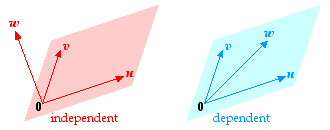
\includegraphics{./mathematics/imgs/linear.png}

A set of vectors is linearly \textbf{dependent} if one of them is \textbf{a linear combination} of the others. (or 0 because you can multiply the other by 0)
